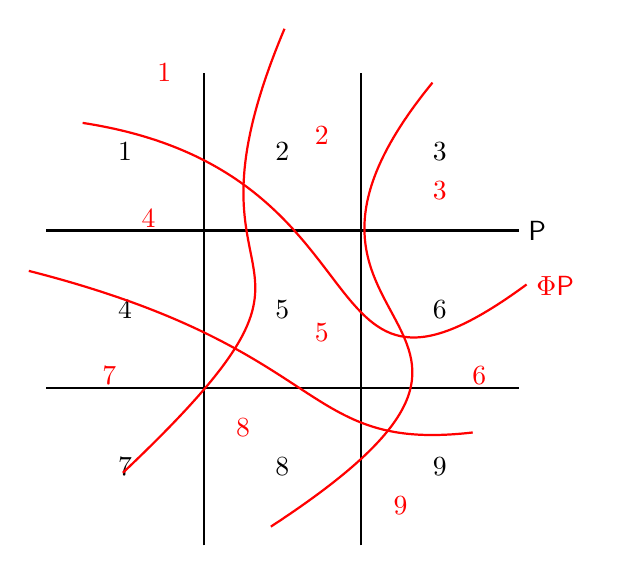
\begin{tikzpicture}
    % Non-transformed grid
    \foreach \t in {2,4} \draw[thick] (\t,0) -- (\t,6);
    \foreach \t in {2,4} \draw[thick] (0,\t) -- (6,\t);
    % Name each cells
    \draw (1,5) node {1}
        (3,5) node {2}
        (5,5) node {3}
        (1,3) node {4}
        (3,3) node {5}
        (5,3) node {6}
        (1,1) node {7}
        (3,1) node {8}
        (5,1) node {9};

    % Transformed grid
    \begin{scope}[red, thick, rotate=-20, yshift=1.2cm, xshift=-1.4cm]
        \foreach \t in {2,4} \draw (\t,0) .. controls ({1 + 1.5*\t},4) and ({1+0.4*\t},2) .. (\t,6);
        \foreach \t in {2,4} \draw (0,\t) .. controls (4,{0 + 1.2*\t}) and (4,1) .. (6,\t);
    \end{scope}
    % Name each new cells
    \draw[red] (1.5,6) node {1}
        (3.5,5.2) node {2}
        (5,4.5) node {3}
        (1.3,4.15) node {4}
        (3.5,2.7) node {5}
        (5.5,2.15) node {6}
        (0.8,2.15) node {7}
        (2.5,1.5) node {8}
        (4.5,0.5) node {9};

    % Labels
    \draw (6,4) node [right] { $ \mathsf{P} $ };
    \draw[red] (6.1,3.3) node [right] { $ \Phi \mathsf{P} $ };
\end{tikzpicture}


